\documentclass[12pt]{article}
\usepackage[utf8]{inputenc}
\usepackage{fancyhdr}
\usepackage[includehead, margin=2cm]{geometry}
\usepackage{listings}
\usepackage{titling}
\usepackage{parskip}
\usepackage{fancyvrb}
\usepackage{tabularx}
\usepackage{float}
\usepackage{mathtools}
\usepackage{hyperref}
\usepackage{graphicx}
\usepackage[normalem]{ulem}

\usepackage{xcolor}
\lstset{basicstyle=\ttfamily,
  showstringspaces=false,
  commentstyle=\color{red},
  keywordstyle=\color{blue}
}
\newcommand{\codeIn}[1]{{\small\tt{#1}}}
\hypersetup{
    colorlinks=true,
    urlcolor=blue
}

\pagestyle{fancy}

\newenvironment{centeredcode}
{
\ttfamily
\begin{center}
\begin{tabular}{l}
}
{
\end{tabular}
\end{center}
}


\newcommand{\classTitle}{CS 6340: Software Analysis and Test}
\newcommand{\projectTitle}{SVF Project}
\newcommand{\implementationFile}{\codeIn{project.cpp} }
\newcommand{\src}{\codeIn{src}}
\newcommand{\sink}{\codeIn{sink}}
\newcommand{\calls}{\xrightarrow[]{calls}}
\newcommand{\returns}{\xrightarrow[]{returns}}


\title{
\classTitle
\Large
\\
\projectTitle
}
\preauthor{}
\postauthor{}
\author{}
\date{}

\begin{document}
\lhead{\classTitle}
\rhead{\projectTitle}
\maketitle
\thispagestyle{fancy}


\section{Project Description}

In this project, you will get familiar with the \href{https://svf-tools.github.io/SVF}{SVF} framework and build a reachability analysis tool for \href{https://llvm.org/docs/LangRef.html#instruction-reference}{LLVM IR}. SVF is a static tool that enables scalable and precise interprocedural dependence analysis on LLVM IRs. Your submitted analysis tool should read LLVM IR files and decide (statically) whether the \sink () function entry block is reachable from the \src () function entry block.



\subsection{Task Description}\label{sec:description}
An interprocedural control-flow graph (ICFG)  describes the control flow of a target program. The ICFG represents the control instructions from the program entry node to the program exit node and provides multiple control flows among the whole program. Analysis of an ICFG can be used to detect path reachability between two nodes. 

\begin{figure*}[htpb]
    \centering
    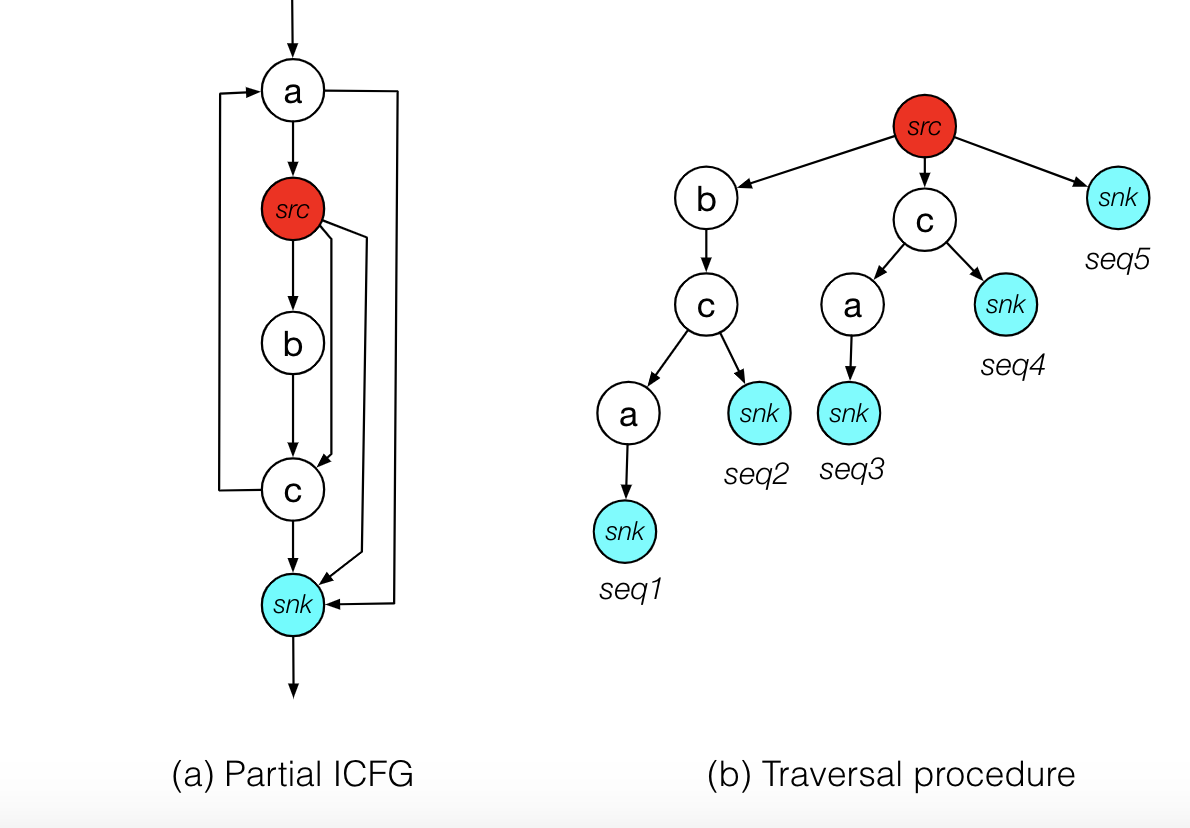
\includegraphics[scale=0.6]{icfgCase1.png}
    \label{case1}
\end{figure*}

\filbreak
Your program should perform the previously mentioned reachability analysis.
Some caveats:
\begin{enumerate}
    \item The analysis should be \textbf{Path-Insensitive \& Context-Sensitive}. \textbf{Be sure to consider how Context-Sensitivity affects your results.} 
    
    \item No data flow analysis is necessary. As such, it is okay to traverse paths that are technically infeasible:
\begin{figure*}[htpb]
    \centering
    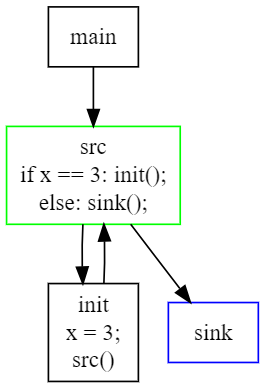
\includegraphics[scale=0.45]{interprocedural.png}
    \label{case2}
\end{figure*}

    \begin{enumerate}
        \item \codeIn{$src \calls sink$} (infeasible)
        \item \codeIn{$src \calls init \returns src \calls sink$}
    \end{enumerate}

\filbreak
    \item There may be multiple call sites of src and sink.
    \begin{center}
        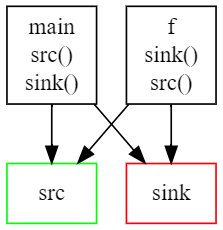
\includegraphics[scale=0.5]
        {multiplecallsites.png}
        \label{case3}
    \end{center}

    \begin{enumerate}
        \item \codeIn{$src \returns main \calls sink$}
    \end{enumerate}

    \item Your analysis should report all cycles within the traversal paths. The connections into the cycle subpath must be correct (the element before the cycle must connect to the first element of the cycle and the element after the cycle must connect to the last element of the cycle). Reporting any of the multiple cyclic representations is fine as long as each cycle is represented in the output. Some additional notes:
    \begin{itemize}
        \item There will be no nested cycles.
        \item Each cycle will have a defining \href{https://llvm.org/docs/LangRef.html#br-instruction}{br instruction} that will not be shared with another cycle.
    \end{itemize}

\begin{figure*}[htpb]
    \centering
    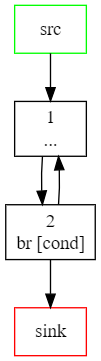
\includegraphics[scale=0.5]{cycles.png}
    \label{case4}
\end{figure*}

    \begin{enumerate}
        \item \codeIn{$src \xrightarrow{} 1 \xrightarrow{} 2 \xrightarrow{} sink$} (acyclic path)
        \item \codeIn{$src \xrightarrow{} Cycle[1 \xrightarrow{} 2] \xrightarrow{} sink$} (cycle path)
        \item \codeIn{$src \xrightarrow{} 1 \xrightarrow{} Cycle[2 \xrightarrow{} 1] \xrightarrow{} 2 \xrightarrow{} sink$} (alternate cycle path)
    \end{enumerate}
    
    \item You do not need to handle indirect function calls
    \item You do not need to handle recursion in callstacks (A function will not call itself anywhere in its body or its sub-functions).
    \item You may end analysis at the \sink () entry node. Paths going through this and eventually reaching the \sink () entry node again do not need to be reported.
    
    
\end{enumerate}
The ICFG can be generated by the SVF framework; SVF also provides the functionality to identify instructions represented by the nodes in the ICFG.

One goal in this project is also to learn how to utilize a real-world static analysis framework to implement analysis tools. Please start early to get familiar with the SVF framework in this project! Reference for the SVF framework is available at \url{https://github.com/SVF-tools/SVF/wiki}. 

\filbreak
\subsection{Project Setup}\label{sec:setup}

\subsubsection{Docker}
To avoid configuration issues, we will use \href{https://www.docker.com/}{Docker} in this project. We provide a guide to use Docker and our grading environment will be the same as described in the guide. Here are the instructions to set up, build, and test your project.

First, you need to install Docker on your local machine. Here is the link to get started with Docker: \url{https://www.docker.com/get-started}.

Once you have Docker installed on your machine, you can pull the provided Docker image from Docker Hub and then work on it. If you want to know more about Docker please consult the official documentation.

\begin{enumerate}
    \item First you can pull the image from Docker Hub.\\\\
    \codeIn{docker pull mdavis438/svfproject:latest}\\
    \item Then you can start a Docker container from the provided Docker image using the following command.\\\\
    \codeIn{docker run -it --name svfproject mdavis438/svfproject:latest /bin/bash}\\\\
    If you want to come back later you can exit the bash session and start the stopped container again using the following command.\\\\
    \codeIn{docker start -ai svfproject}\\\\
\end{enumerate}

\textbf{Please keep in mind that docker containers will not save changes when closed! Either:
\begin{enumerate}
    \item Save the container to a docker image
    \item Mount the project directory to your local computer \\(add \codeIn{-v host/directory/path:/home/project/src} to your docker run command)
    \item Save the file copy to your local machine before closing the container
    \item Save your code on a private repository
\end{enumerate}
}

\filbreak
\subsubsection{VSCode (optional)}

This section provides a guide for if you want to use VScode dev container connections.

\begin{enumerate}
    \item Install VSCode Editor: \url{https://code.visualstudio.com/download}

    \item Install Remote Development Extension in VSCode

    \begin{center}
        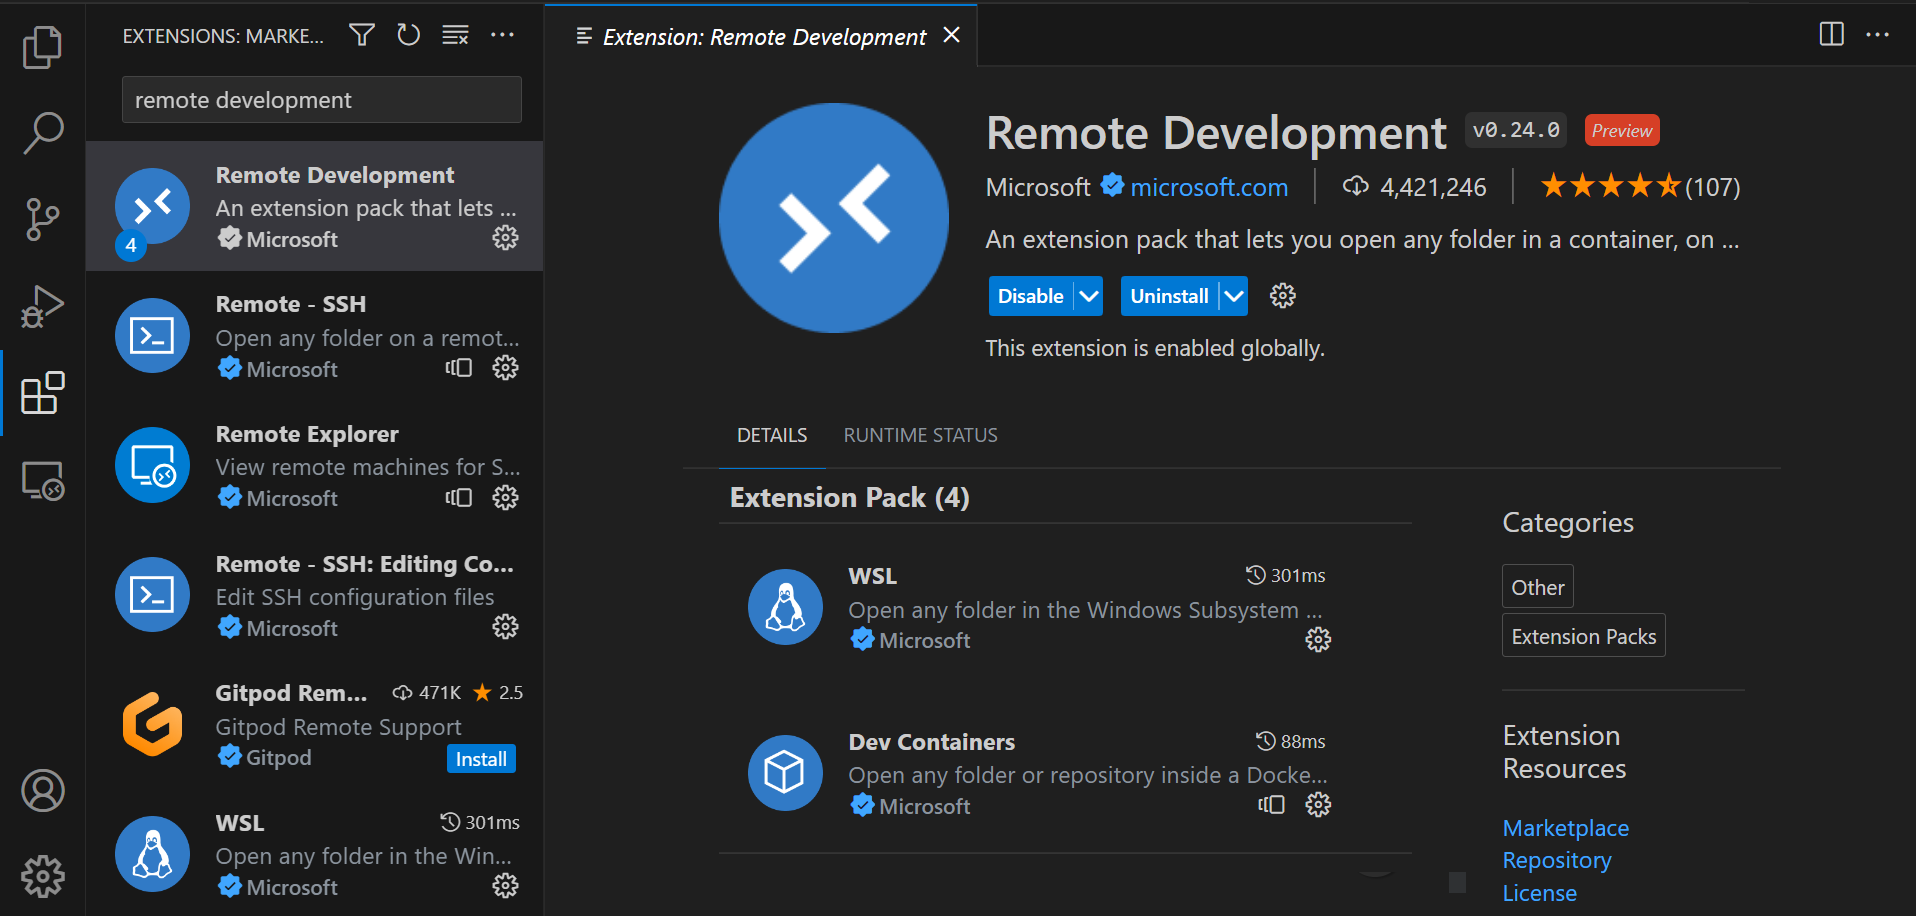
\includegraphics[width=0.8\linewidth]{extension.png}
        \label{fig:install_docker}
    \end{center}

    \item This alternative of the docker start command will start the container in the background without an interactive terminal:\\
    \codeIn{docker start svfproject}

    \item Attach to the docker container. 
    
    Open the Remote Explorer view from the left panel. Select "Dev Containers" in the dropdown at the top of the sidebar. This should list all of the docker containers available.
    
    Choose your project container ('svfproject'). VSCode will take some time to setup the connection and then open the container environment.
    
    \begin{center}
        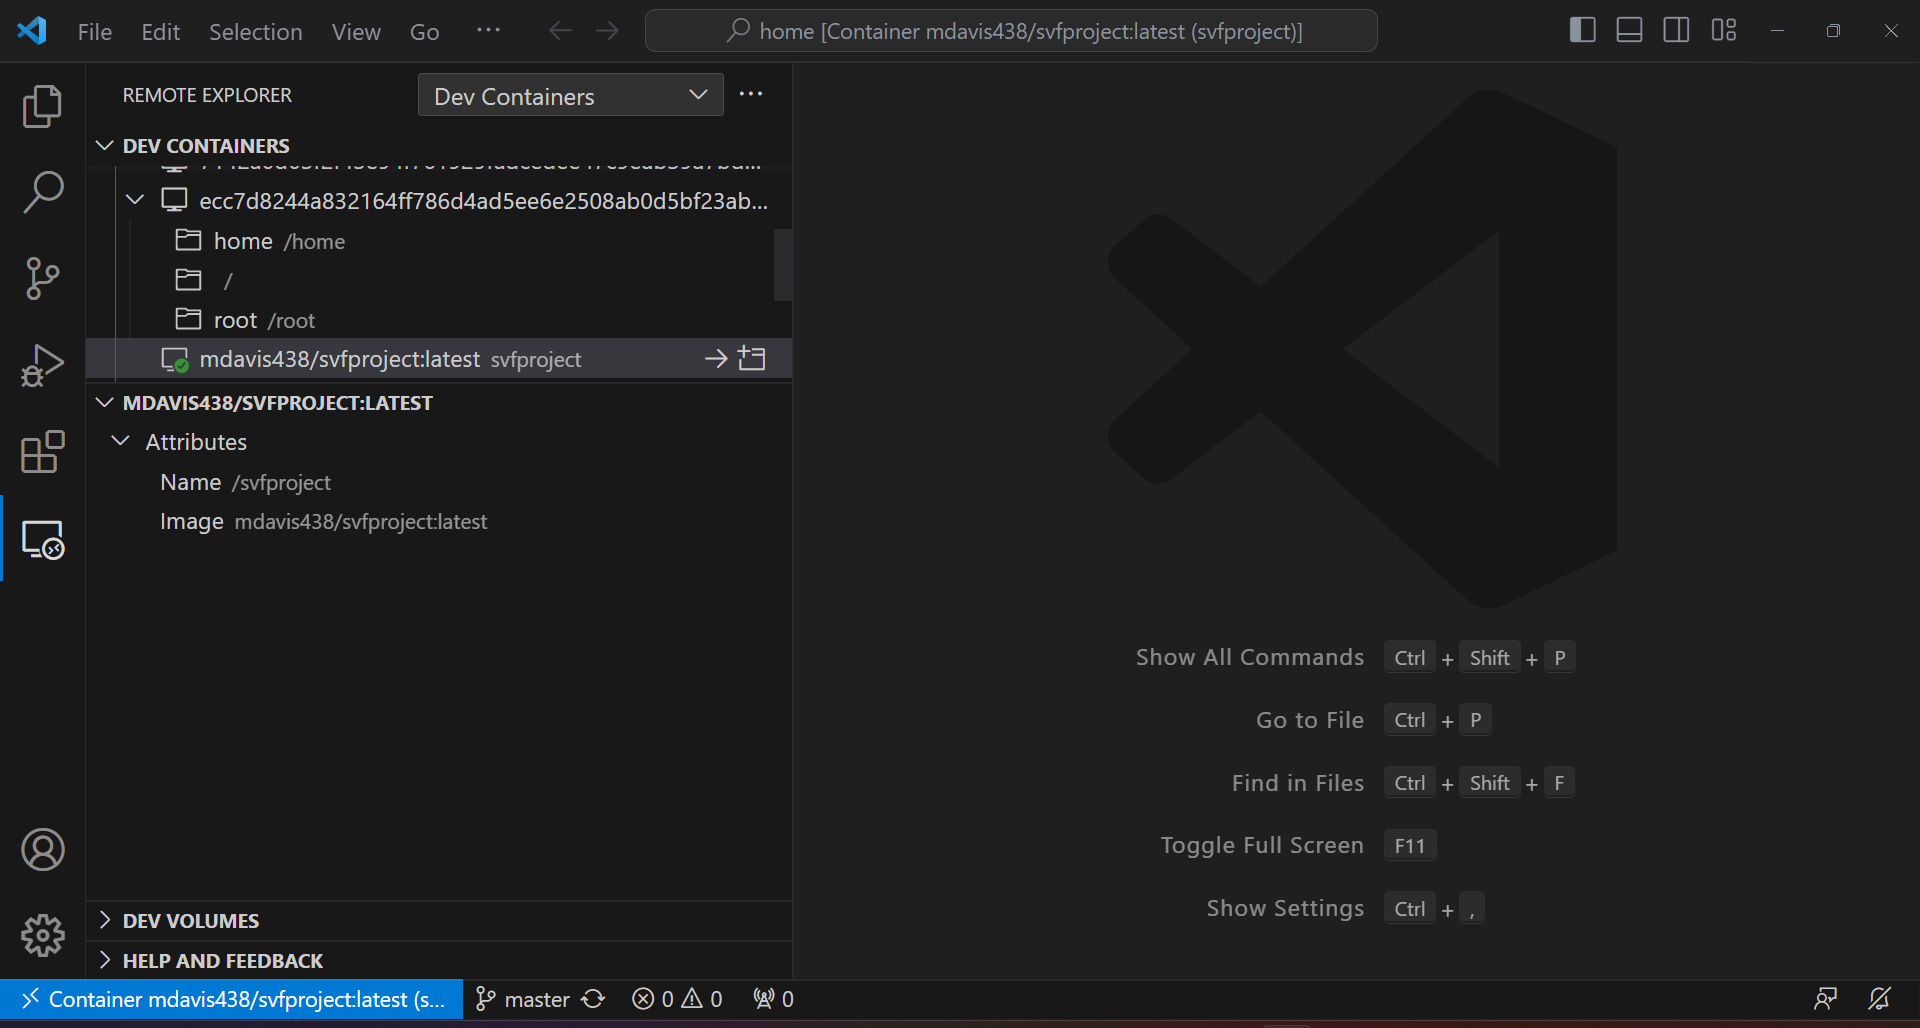
\includegraphics[width=0.8\linewidth]{attach.png}
        \label{fig:attach}
    \end{center}
    
    More info on dev containers can be found \href{https://code.visualstudio.com/docs/devcontainers/containers}{here}. VSCode provides this \href{https://code.visualstudio.com/docs/devcontainers/tutorial}{tutorial} but be sure to replace the example container instructions with our docker container.
    
\end{enumerate}

\subsubsection{Project Setup}
\begin{enumerate}
    \item To complete this project, you only need to modify the following file inside the container.\\\\
    \codeIn{$\sim$/project/src/project.cpp}\\
    
    \item After completing the code in this file you can build the project by first going to the directory ``\codeIn{$\sim$/project/}'' and then running the following commands\\\\
    \codeIn{source ./env.sh}\\
    \codeIn{./build.sh}\\

    \item This will generate the executable \codeIn{$\sim$/project/bin/svf-project}. The project can be run using the command\\\\    
    \codeIn{./test.sh [path/to/test.bc]}\\\\
    and will generate the \codeIn{out.txt} output file
    

\end{enumerate}
\section{Provided Code}

The provided code and test case information is in the Docker container on Docker Hub. In the Docker container we have provided the framework to build the project based on the dependence of SVF libraries. In the placeholder \implementationFile file, you need to perform the reachability analysis and print the result to \codeIn{stdout}. There are also many test cases provided in \codeIn{$\sim$/project/test\_cases}.

\section{Grading}
There are in total 100 points for this project.

\subsection{Correct Implementations (60 Points)}

Several test cases are given to you to test the correctness of your project under the \codeIn{$\sim$/project/test\_cases} directory. You can run the script \codeIn{test.sh} and compare your output to the README file in the \codeIn{$\sim$/project/test\_cases} directory to check the correctness of your implementation. For grading, there will be hidden test cases for the project. \textbf{The provided example test cases DO NOT fully cover the possibilities of the problem which may appear in the hidden test cases. It is highly recommended to thoroughly test your implementation by writing your own tests.} We will use the build.sh script to build your project, and there will be no optimizations or transformations performed on the IR you will be graded on (no loop unrolling etc.)

For each input test case, your program is expected to print out the following outputs:
\begin{itemize}
    \item \textbf{First line - 40 Points:} The result whether the function entry block of \src () can reach the function entry block of \sink (). If it is reachable, your program should print ``Reachable'', otherwise print  ``Unreachable''. Print the EXACT text of ``Reachable'' or ``Unreachable''. You will receive the proportion of 40 Points corresponding to the proportion of matching reachability results in the hidden testcases.
    \item \textbf{Following lines - 20 Points:} If there are $n$ traversal paths between the \src\  and \sink, your project should also print $n$ more lines. Each line 
    is a path from \src () to \sink (). The path should report the ICFG Node IDs in order of the path, starting with the func entry node of \src () and ending with the func entry node of \sink () (specifically the nodes returned via \codeIn{FunEntryICFGNode* getFunEntryICFGNode(const SVFFunction* fun);}).
    
    Supposing that node 1 is the \src\  node and node 5 is the \sink\  node, a path could look like: \codeIn{$1\xrightarrow{}2\xrightarrow{}3\xrightarrow{}4\xrightarrow{}5$}. 
    
    In the instance that the path or a portion is cyclic, annotate the cyclic region in the format described in~\ref{sec:description}. Example: \codeIn{$1\xrightarrow{}Cycle[2\xrightarrow{}3\xrightarrow{}4]\xrightarrow{}5$}. The entry/exit nodes from the cycle must be correct, regardless if this duplicates nodes i.e. \codeIn{$1\xrightarrow{}Cycle[2\xrightarrow{}3\xrightarrow{}4\xrightarrow{}2]\xrightarrow{}5$}. In general, if there is a cycle, make sure it is reported in at least one path. Some cycles can have multiple representations, but as long as one of the variations is reported that is sufficient.
    
    Correct program traversal paths will award 20 Points.
\end{itemize}

\subsection{Performance Evaluation (10 Points)}\label{sec:eval}
If your program can finish running each test case in 30 seconds, you will get 10 Points. The test cases are incredibly small (max of $\approx$300 nodes). If your analysis takes over 30 seconds for a test this is probably an extreme time complexity problem with your implementation.

\subsection{Design (30 Points)}\label{sec:design}

In your final report, 
please briefly describe the following:
%
\begin{enumerate}
\item Details about how you perform the reachability analysis.
\item Details about how you perform the cycle detection.
\item Details about how you made the analysis context-sensitive and how this affects the results.
\item Any known outstanding bugs or deficiencies that were unable to be resolved before submission.
\item "Future work"-style ways that the analysis could be improved or extended.
 \end{enumerate}

\section{Submission}\label{sec:sub}
As stated before, to facilitate the grading, you should not modify other files besides \codeIn{project.cpp} in the project directory!
On Canvas, submit a single ZIP file that contains:
\begin{itemize}
    \item The \implementationFile file
    \item The \codeIn{design.pdf} file described in Section~\ref{sec:design}.
    \item Any test cases you added (these will not be graded).
\end{itemize}
\textbf{We will only use the \implementationFile file to test the correctness of your implementation. If you modify other files, even if your code runs correctly on your local machine, you will still get points deducted if it cannot run properly in our grading environment.}

\section{Collaboration}
%
We will award identical grades to each member of a given project team, unless members of the team directly register a formal complaint.
%
We assume that the work submitted by each team is their work solely.
% 
Any questions about design and implementation should conducted solely with the instructors through office hours, email, etc.
%
Under no condition is it acceptable to use code written by another team, or obtained from any other source.
%
As part of the standard grading process, each submitted solution will automatically be checked for similarity with other submitted solutions and with other known implementations.

\end{document}
